\documentclass[8pt,letterpaper]{article}
\usepackage{graphicx}

\begin{document}
\title{A random walker world map generator}
\maketitle

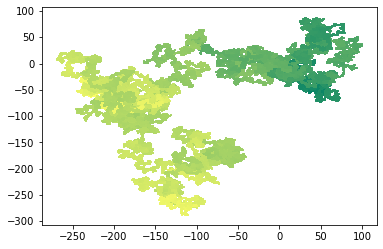
\includegraphics{Images/random_walker_world.png}
\newpage{}
\section{Introduction}
The random walker algorithm is created with the goal to create a random movement generator. by marking the spots where the walker has visited a world map can be generated in a simple way. The walker used in this test is a 3d walker. 

\section{How does it work}
The first two dimensions(x and y axis) are used to create a 2d map. The 3rd dimension(color axis) is used to create color in the map. The values are then placed over a color gradient and each pixel is given a color value based on the position of the map. In the case of this world map green to yellow was used as a gradient. The walker will randomly select x, y and colour values. The walker will do this 100.000 times to create a large amount of variation.

The order of action is:

\begin{enumerate}
	\item Start a random walker with an x, y and colour value set;
	\item Change both the X Y and colour value by 1 at random(can not change as well, but at least the x or y value has to change to prevent useless changes. The changes are saved in a numpy array (example :[[x1, y1, colour1],[x2,y2,colour2]]);
	\item Repeat the previous step 100.000 times;
	\item Plot the values using a graphic program(pyplot is used by me);
	\item add a colour gradient and plot the colour values on it(lowest value is the bottom of gradient, highest is top, etc).
\end{enumerate}
\section{The advantages}
The advantages of the random walker are:
\begin{itemize}
    \item A fast method to create worlds
        \begin{itemize}
        \item Fast loading times;
        \item Easy to create;
        \item Low processor power required.
        \end{itemize}
    \item simple but nice looking worlds
\end{itemize}
\section{The disadvantages}
The disadvantages of the random walker are
\begin{itemize}
    \item low adaptability
    \item no control over world generation
    \item Changing sprite work is near impossible
\end{itemize}

\section{conclusion}
The method is fun for simple world generation but is not usable for how advanced I want the world creator to be, therefore this method will not be used in the last version. Perlin noise might have similarities with this method that will be used in later versions of this generator.

\end{document}



